% GoethitePaper_SI.tex -- Supplementary Information wrapper for GoethitePaper.tex.
% Built by Chapter2/Paper/build_paper_from_chapter2.py (2026-11-02).
\documentclass[preprint,12pt,authoryear]{elsarticle}
\journal{Geochimica et Cosmochimica Acta}
\usepackage{lmodern}
\usepackage[T1]{fontenc}
\usepackage[utf8]{inputenc}
\usepackage{graphicx}
\usepackage{amsmath}
\usepackage{amssymb}
\usepackage{array}
\usepackage{booktabs}
\usepackage{longtable}
\usepackage{subcaption}
\usepackage{lineno}
\usepackage{xr}
\usepackage{xurl}
\usepackage[colorlinks=true,linkcolor=blue,citecolor=blue,urlcolor=blue]{hyperref}
\graphicspath{{../Figures/source/}{../Figures/generated/}}
% =============================================================
%  chapter2_derived_values.tex -- AUTO-GENERATED, DO NOT EDIT BY HAND.
%  Written by Figures/write_chapter2_macros.py from
%  Figures/generated/data/stage1_regression_cache.json (itself written by
%  Figures/prepare_regression_cache.py from the master workbook).
%
%  Regenerate after any data/regression change:
%    python3 Figures/prepare_regression_cache.py
%    python3 Figures/write_chapter2_macros.py
%  (run_all_figures.py does both automatically.)
%
%  \input{} by BOTH chapter2goethite.tex (standalone) and
%  Chapter2/chapter2.tex (dissertation chapter) so the Abstract,
%  Results, Discussion, and Conclusions all read the same numbers.
%
%  Stage 1 reference line (3He, "treatment as uncertainty" central/M
%  bound, fractional 3He yield >= 0.07, n=12 points, R2=0.9890):
%    ChTwoEa/ChTwoEaErr : activation energy (kJ/mol)
%    ChTwoTc/ChTwoTcErr : Dodson (1973) closure temperature (degC),
%      intercept-only regression uncertainty (D0/a^2 term only, Ea
%      held fixed) -- see thermochr_utils.dodson_closure_temperature_stderr_interceptonly.
%      Joint slope+intercept uncertainty is +/- 14.9 degC if ever needed.
%    ChTwoRtwo/ChTwoN   : regression R^2 and number of points
%
%  Isothermal 3He permeation Arrhenius regression (from
%  generated/data/naive_lambda_arrhenius_cache.json, n=10 sequences, R2=0.9362):
%    ChTwoPermEa/ChTwoPermEaErr : activation energy, 2 s.e. (cal/mol)
%    ChTwoPermRtwo/ChTwoPermN   : regression R^2 and number of sequences
% =============================================================
\newcommand{\ChTwoEa}{157.1}
\newcommand{\ChTwoEaErr}{5.3}
\newcommand{\ChTwoTc}{98.1}
\newcommand{\ChTwoTcErr}{8.6}
\newcommand{\ChTwoRtwo}{0.989}
\newcommand{\ChTwoN}{12}
\newcommand{\ChTwoPermEa}{10192}
\newcommand{\ChTwoPermEaErr}{1882}
\newcommand{\ChTwoPermRtwo}{0.936}
\newcommand{\ChTwoPermN}{10}

% =============================================================
%  chapter2_kinetics_values.tex -- AUTO-GENERATED, DO NOT EDIT BY HAND.
%  Written by Chapter2/Figures/fig_goethite_vacuum_kinetics.py
%  (write_kinetics_macros) from the kinetic fits to the vacuum step heats
%  (KAF = Farley et al. 2024; HDM = Monteiro et al. 2017). Statistics cache:
%  Figures/generated/data/goethite_kinetics_cache.json.
%  Rerun that script (or run_all_figures.py) after any change to the data
%  or fitting code.
% =============================================================
\newcommand{\ChTwoKinFOneEa}{120.8}
\newcommand{\ChTwoKinFOneLnA}{18.15}
\newcommand{\ChTwoKinPhi}{0.101}
\newcommand{\ChTwoKinS}{0.47}
\newcommand{\ChTwoKinFOneRmsKAF}{0.0087}
\newcommand{\ChTwoKinFOneRmsHDM}{0.018}
\newcommand{\ChTwoKinNKAF}{18}
\newcommand{\ChTwoKinNHDM}{19}
\newcommand{\ChTwoKinWinKAF}{5--22}
\newcommand{\ChTwoKinWinHDM}{8--26}
\newcommand{\ChTwoKinWinKAFT}{185--280}
\newcommand{\ChTwoKinWinHDMT}{180--296}
\newcommand{\ChTwoKinDThreeEa}{196}
\newcommand{\ChTwoKinDThreeRmsKAF}{0.039}
\newcommand{\ChTwoKinDThreeRmsHDM}{0.048}
\newcommand{\ChTwoKinDThreeRmsRatio}{4.4}
\newcommand{\ChTwoKinDThreePhiEa}{243}
\newcommand{\ChTwoKinDThreePhiRmsKAF}{0.026}
\newcommand{\ChTwoKinDThreePhiRmsHDM}{0.056}
\newcommand{\ChTwoKinDThreePhiRmsRatio}{3.0}
\newcommand{\ChTwoKinDThreePhiS}{1.00}
\newcommand{\ChTwoKinDThreeFreeEa}{289}
\newcommand{\ChTwoKinDThreeFreePhi}{0.184}
\newcommand{\ChTwoKinDThreeFreeRmsKAF}{0.019}
\newcommand{\ChTwoKinDThreeFreeRmsHDM}{0.052}
\newcommand{\ChTwoKinWaterEa}{90.9}
\newcommand{\ChTwoKinWaterRms}{0.034}
\newcommand{\ChTwoKinAllFOneEa}{122.7}
\newcommand{\ChTwoKinAllPhi}{0.112}
\newcommand{\ChTwoKinAllFOneRmsKAF}{0.0073}
\newcommand{\ChTwoKinAllFOneRmsHDM}{0.026}
\newcommand{\ChTwoKinAllRThreeEa}{99.4}
\newcommand{\ChTwoKinAllRThreeRmsKAF}{0.0097}
\newcommand{\ChTwoKinAllRThreeRmsHDM}{0.030}
\newcommand{\ChTwoKinAllRTwoEa}{87.9}
\newcommand{\ChTwoKinAllRTwoRmsKAF}{0.012}
\newcommand{\ChTwoKinAllRTwoRmsHDM}{0.033}
\newcommand{\ChTwoKinAllDThreeEa}{177.4}
\newcommand{\ChTwoKinAllDThreeRmsKAF}{0.063}
\newcommand{\ChTwoKinAllDThreeRmsHDM}{0.062}
\newcommand{\ChTwoKinAllDThreePhiRmsKAF}{0.022}
\newcommand{\ChTwoKinAllDThreePhiRmsHDM}{0.042}
\newcommand{\ChTwoKinLineEa}{137.0}
\newcommand{\ChTwoKinLineEaErr}{2.7}
\newcommand{\ChTwoKinLineLnA}{21.91}
\newcommand{\ChTwoKinLineLnAErr}{0.66}
\newcommand{\ChTwoKinLineN}{35}
\newcommand{\ChTwoKinKAFEa}{139.3}
\newcommand{\ChTwoKinKAFEaErr}{6.2}
\newcommand{\ChTwoKinHDMEa}{135.4}
\newcommand{\ChTwoKinHDMEaErr}{2.5}
\newcommand{\ChTwoKinKTwoFifty}{6.8\times10^{-5}}
\newcommand{\ChTwoKinConvPerHour}{22}
\newcommand{\ChTwoKinCeiling}{63}
\newcommand{\ChTwoKinDetect}{9}
\newcommand{\ChTwoKinPhiPct}{10}
\newcommand{\ChTwoKinOneMinusPhi}{0.899}
\newcommand{\ChTwoKinHTFEnd}{0.147}
\newcommand{\ChTwoKinHTAlphaObs}{0.16}
\newcommand{\ChTwoKinLogAlphaLow}{-12.4}
\newcommand{\ChTwoKinLogAlphaMid}{-20.7}
\newcommand{\ChTwoKinLogAlphaHigh}{-25.8}
\newcommand{\ChTwoKinAlphaPermissive}{2\times10^{-3}}
\newcommand{\ChTwoKinTrapSuppLow}{0.33}
\newcommand{\ChTwoKinTrapSuppHigh}{0.22}
\newcommand{\ChTwoKinResidRmsKAF}{0.11}
\newcommand{\ChTwoKinResidRmsHDM}{0.07}
\newcommand{\ChTwoKinTrapResidLow}{0.34}
\newcommand{\ChTwoKinTrapResidHigh}{0.63}
\newcommand{\ChTwoKinSumKdt}{60}
\newcommand{\ChTwoKinLogRDetect}{-3.8}
\newcommand{\ChTwoKinLogRObs}{-2.5}
\newcommand{\ChTwoKinNMC}{4000}
\newcommand{\ChTwoKinCNTLogRLo}{-28.4}
\newcommand{\ChTwoKinCNTLogRHi}{-14.0}
\newcommand{\ChTwoKinCNTLogAlphaLo}{-26.7}
\newcommand{\ChTwoKinCNTLogAlphaHi}{-12.3}
\newcommand{\ChTwoKinMCCNTLo}{-38.7}
\newcommand{\ChTwoKinMCCNTMid}{-18.8}
\newcommand{\ChTwoKinMCCNTHi}{-9.1}
\newcommand{\ChTwoKinGammaLo}{0.12}
\newcommand{\ChTwoKinGammaHi}{0.15}
\newcommand{\ChTwoKinMCGammaLo}{0.12}
\newcommand{\ChTwoKinMCGammaHi}{0.15}
\newcommand{\ChTwoKinMCGammaMid}{0.14}
\newcommand{\ChTwoKinSLowRange}{0.30--0.37}
\newcommand{\ChTwoKinSHighRange}{0.22--0.23}
\newcommand{\ChTwoKinRstarVac}{0.00--0.00}
\newcommand{\ChTwoKinRstarSat}{0.7--0.9}
\newcommand{\ChTwoKinNfuVac}{0.00--0.00}
\newcommand{\ChTwoKinNfuSat}{26--52}
\newcommand{\ChTwoKinBarVac}{0.0--0.0}
\newcommand{\ChTwoKinBarSat}{32--63}
\newcommand{\ChTwoKinBarReq}{18}
\newcommand{\ChTwoKinGammaMin}{0.10}
\newcommand{\ChTwoKinGammaTwin}{0.24}
\newcommand{\ChTwoKinGammaRatio}{2.4}
\newcommand{\ChTwoKinAlphaTarget}{10^{-6}}
\newcommand{\ChTwoKinRstarMin}{0.56}
\newcommand{\ChTwoKinNfuMin}{14}
\newcommand{\ChTwoKinBarMin}{18}
\newcommand{\ChTwoKinRstarTwin}{1.4}
\newcommand{\ChTwoKinNfuTwin}{212}
\newcommand{\ChTwoKinBarTwin}{259}
\newcommand{\ChTwoKinLogAlphaTwin}{-111}
\newcommand{\ChTwoKinMechFitRows}{R2 & 92.8 & 10.63 & 0.149 & 0.0133 & 0.0291 \\ R3 & 103.1 & 12.73 & 0.136 & 0.0114 & 0.0240 \\ F1 & 120.8 & 18.15 & 0.101 & 0.0087 & 0.0176 \\ A2 & 25.5 & $-4.73$ & 0.000 & 0.0212 & 0.1906 \\ A3 & 20.0$^{a}$ & $-5.85$ & 0.203 & 0.0433 & 0.2342 \\ D3, $\phi=0$ & 195.6 & 32.43 & 0.000 & 0.0385 & 0.0484 \\ D3, $\phi=\phi_{\mathrm{F1}}$ & 242.8 & 43.91 & 0.101 & 0.0258 & 0.0557 \\ D3, $\phi$ free & 288.5 & 55.04 & 0.184 & 0.0186 & 0.0520 \\}
\newcommand{\ChTwoKinSynthRows}{R2 & 140.0 & 0.0031 & 140.4 & 0.0028 \\ F1 & 173.0 & 0.0074 & 177.4 & 0.0092 \\ A2 & 81.7 & 0.0073 & 83.8 & 0.0077 \\ A3 & 51.3 & 0.0073 & 53.8 & 0.0062 \\ D3 & 296.2 & 0.0026 & 296.9 & 0.0025 \\ R3 (true) & 150.0 & 0.0000 & 150.0 & 0.0000 \\}

% Auto-generated by Figures/fig_winsor_mdd_report.py -- do not edit by hand
\newcommand{\MDDDomainTableRows}{1 & 85.30 & 27.45 & 0.0 & 100.0 & 0.80 \\ 2 & 20.20 & 3.30 & 2.2 & 97.8 & 1.05 \\ 3 & 8.45 & 1.08 & 2.7 & 97.3 & 1.12 \\ 4 & 7.81 & 1.00 & 2.8 & 97.2 & 1.12 \\ 5 & 7.81 & 1.11 & 2.8 & 95.1 & 1.12 \\ 6 & 7.81 & 1.24 & 2.8 & 85.6 & 1.12 \\ 7 & 7.81 & 1.40 & 2.8 & 85.3 & 1.12 \\ 8 & 7.81 & 1.62 & 2.8 & 76.8 & 1.12 \\ 9 & 7.81 & 1.91 & 2.8 & 76.5 & 1.12 \\ 10 & 7.81 & 2.34 & 2.8 & 74.6 & 1.12 \\}
\newcommand{\MDDThermalTableRows}{Linear cooling & 150 & 150 & 78 & 2.00 & 132 & 150--175 & 150--175 & 76--80 \\ Burial & 180 & 70 & 61 & 5.36 & 164 & fixed & 60--82 & 58--65 \\ Burial & 195 & 80 & 61 & 5.04 & 177 & fixed & 68--98 & 58--65 \\ Burial & 210 & 115 & 71 & 6.53 & 180 & fixed & 105--130 & 70--74 \\ Isothermal hold & 150 & -- & 41 & 18.5 & 141 & 140--190 & -- & 39--43 \\}
\newcommand{\MDDFreeNmax}{10}
\newcommand{\MDDNfit}{24}
\newcommand{\MDDNkeep}{28}
\newcommand{\MDDNsteps}{34}
\newcommand{\MDDLinGlobalChi}{1.68}
\newcommand{\MDDLinGlobalT}{89}
\newcommand{\MDDLinGlobalTform}{80}
\newcommand{\MDDLinGlobalAge}{68}
\newcommand{\MDDIsoChi}{18.5}

\providecommand{\hl}[1]{#1}
\externaldocument{GoethitePaper}
\externaldocument[ch1-]{../../Chapter1/Writing/TubeMethodPaper}
\externaldocument[ch1-]{../../Chapter1/Writing/SI}
\renewcommand{\thesection}{S\arabic{section}}
\renewcommand{\thetable}{S\arabic{table}}
\renewcommand{\thefigure}{S\arabic{figure}}
\renewcommand{\theequation}{S\arabic{equation}}

\begin{document}

\nolinenumbers

\begin{frontmatter}
\title{Supplementary Information for: Helium Step Heats on Goethite at Water Saturated Conditions Show Diffusive Helium Loss and High Retentivity at Surface Temperatures}
\author[caltech]{Ben J. Thyer\corref{cor1}}
\ead{benjthyer@gmail.com}
\author[caltech]{Jonathan Treffkorn}
\author[caltech]{Kenneth A. Farley}
\cortext[cor1]{Corresponding author.}
\affiliation[caltech]{organization={Division of Geological and Planetary Sciences, California Institute of Technology},
            city={Pasadena}, postcode={91125}, state={CA}, country={USA}}
\end{frontmatter}

% Built by Chapter2/Paper/build_paper_from_chapter2.py -- see PORT_CHANGELOG.md

\section{Permeation Lag Correction and Ampoule Permeability}\label{sec:ch2-si-permeation}

\subsection{Permeation Lag Correction}\label{permeation-lag-correction}

Because HT-Win-06-01b was encapsulated in an imperfectly
helium-transmissive silica glass ampoule, permeation lag was an expected complication in these
measurements. To address this, experimental steps at temperatures at or above 170°C were bracketed by low temperature
(\textless120°C) steps where the helium in goethite at high pH2O was
effectively immobile at experimental timescales, following the permeation step method of \citet{thyer2026method}. For \textsuperscript{3}He, measured
signals at these low temperature permeation steps were entirely
controlled by the process of permeation through silica glass, and
therefore could be used to estimate the amount of helium remaining within the
ampoule between high-temperature experimental steps. However, for \textsuperscript{4}He,
the measured signals at low temperature permeation steps were most often
indistinguishable from the blank, so Eq.~\eqref{ch1-eq:n0perm} of \citet{thyer2026method} could not be
applied to \textsuperscript{4}He and the permeation step method could not be carried through for that isotope.

As a result, permeation lag is instead addressed using the bounding method described in \citet{thyer2026method}, which constrains the ampoule's residual helium from above rather than measuring it.
In this approach, an upper bound constraint for the helium content of the ampoule at the end of each high-temperature step was
calculated using Eq.~\eqref{ch1-eq:steadystate} of \citet{thyer2026method}. \textsuperscript{3}He was reduced this way as well, for consistency with \textsuperscript{4}He; because \textsuperscript{3}He can also be reduced by the permeation step method, the two reductions can be compared directly; that comparison, an internal test of the bounding method, is given by \citet{thyer2026thesis}.

Both routes require the ampoule's permeation rate constant $\lambda$, which was measured during the experiment itself rather than assumed from the literature (\citealt{thyer2026method}). This in-experiment measurement is not an alternative method of handling permeation lag but a prerequisite of the permeation step method and, here, the empirical basis for choosing a conservative $\lambda$ for the bounding method. It is indispensable in this experiment: the permeability of ampoules used in water vapor saturated step heats
cannot reasonably be assumed to match literature values for anhydrous silica glass.

Ten series of 3--4 consecutive permeation steps held at a single
temperature between 90--110°C for 120-180 minutes each with 26 minutes of
cooling time before being inlet into the Helix-MC-Plus\textsuperscript{10K} were
identified as suitable for this exercise. The \textsuperscript{3}He measurements in these
series were fit to Eq.~\eqref{ch1-eq:incyield} of \citet{thyer2026method} using a non-linear least
squares optimization (Fig.~\ref{fig:ch2-permeation-fits}). This is accomplished with
the Levenberg-Marquardt algorithm implemented in
the curve\_fit function in the SciPy package of Python
\citep{virtanen2020}, weighted by each measurement's own uncertainty.
One additional series that otherwise qualified was not well fit by this
model and was not used further for clarity, though its fit value of
$\lambda$ was within uncertainty of the other series' fit values for
$\lambda$.

An initial guess of $\lambda$ $\approx$ 6$\times$10\textsuperscript{-6}
sec\textsuperscript{-1} and \(n_{0} \approx \frac{m_{i}}{1 - e^{- \lambda t_{i}}}\)
(evaluated at the first measurement of a series) pccSTP was passed to
the optimizer for each series. Uncertainties from the model fits were
calculated using the covariance matrices generated for each of the model
fits. Although the initial helium amount \(n_{0}\) was a free parameter
in the optimizations, the rate constant of permeation ($\lambda$) was
the only parameter of interest for this exercise. The fitted rate constants span
\ChTwoPermLamMin\ to \ChTwoPermLamMax\ s\textsuperscript{-1}, with 2$\sigma$ uncertainties of
0.08 to 0.46 log units and no trend resolvable against step duration:

\begin{figure}[htbp]
\centering
\includegraphics[width=0.8\textwidth]{PermeationStepFits_Grid.pdf}
\caption{Cumulative yield against cumulative time for helium-3 yields for isothermal permeation steps. A non-linear least squares optimization fits $\lambda$ and $n_0$ of Eq.~\eqref{ch1-eq:incyield} of \citet{thyer2026method} to data from a series of permeation steps like these. The permeability $K$ is calculated according to the relation $K = \lambda/GRT$ and is plotted as a function of temperature in Fig.~\ref{fig:ch2-ampoule-permeability}. The curvature of each series is what conditions the fit: a series in which the permeation rate has not yet slowed appreciably constrains $\lambda$ and $n_0$ only weakly.}
\label{fig:ch2-permeation-fits}
\end{figure}

\begin{figure}[htbp]
\centering
\includegraphics[width=0.8\textwidth]{AmpoulePermeability_Arrhenius.pdf}
\caption{Arrhenius plot of apparent permeation coefficients as a function of inverse temperature for HT-Win-06-01b, converted from the rate constants fitted in Fig.~\ref{fig:ch2-permeation-fits} via $K = \lambda/GRT$. The activation energy is higher than anhydrous silica glass, as expected \citep{masaryk1968,shelby1972}. It is unexpected that the glass ampoule of HT-Win-06-01b has higher apparent \textsuperscript{3}He permeability than the literature values of \citet{swets1961} and \citet{jones1953}, but this can be explained by an increase in the partial pressure of the gas phase within the tube due to displacement by high He diffusivity, low He solubility water. Yellow points labeled ``Diffusion Model with cooling, Anhydrous'' were produced to evaluate the expected excess apparent permeability due to the 25 minute cooldown period before measurement. This is accomplished by simulating the measured apparent permeability for a dry silica glass ampoule that continued to permeate helium while cooling for an additional 26 minutes before measurement after being held at 90--110\textdegree C for 120--180 minutes, similarly to the measured values. Variability in these points is due to differences in the length of time the ampoule was heated but is very small. They show a near constant offset from the expected values of \citet{swets1961} and \citet{jones1953} that is much smaller than the uncertainty in the regression of the fit values determined experimentally in teal.}
\label{fig:ch2-ampoule-permeability}
\end{figure}

All measured apparent \textsuperscript{3}He permeabilities were equal to or in excess of the literature values for anhydrous silica glass (Fig.~\ref{fig:ch2-ampoule-permeability}),
similar to observations discussed in \citet{thyer2026method}. \textsuperscript{4}He permeability itself could not be independently measured in this
experiment due to blank-level signals during the low temperature permeation steps and is assumed to similarly exceed the literature values for anhydrous silica glass.
To evaluate the uncertainty due to the permeation lag, we use the literature values as a conservative (lower bound) estimate of the true permeability; a $\lambda$ that underestimates the ampoule's true rate constant yields a conservative (higher) upper bound on the residual helium (\citealt{thyer2026method}).
$\lambda t$ (where $\lambda = GRTK$) is estimated here using the \textsuperscript{4}He
permeability \emph{K} reported by \citet{swets1961}, while the \textsuperscript{3}He permeability
is taken to be the product of the \textsuperscript{4}He permeability and the relative \textsuperscript{3}He/\textsuperscript{4}He permeability reported by \citet{jones1953}. The geometric constant \emph{G} is calculated using the measured inner and
outer diameter of the ampoule (Fig.~\ref{fig:ch2-ampoule-dims}).

The first three experimental steps had values of $\lambda t$ lower than 4, and therefore
the upper bound of the helium content of these steps could not be determined. These measurements are omitted
from further analysis. Later experimental steps with values of $\lambda t$ lower than 4 could be determined
using Eq.~\eqref{ch1-eq:s6-8} from the supplement to \citet{thyer2026method} because upper bounds on previous steps' residual helium
content could be evaluated.

\begin{figure}[htbp]
\centering
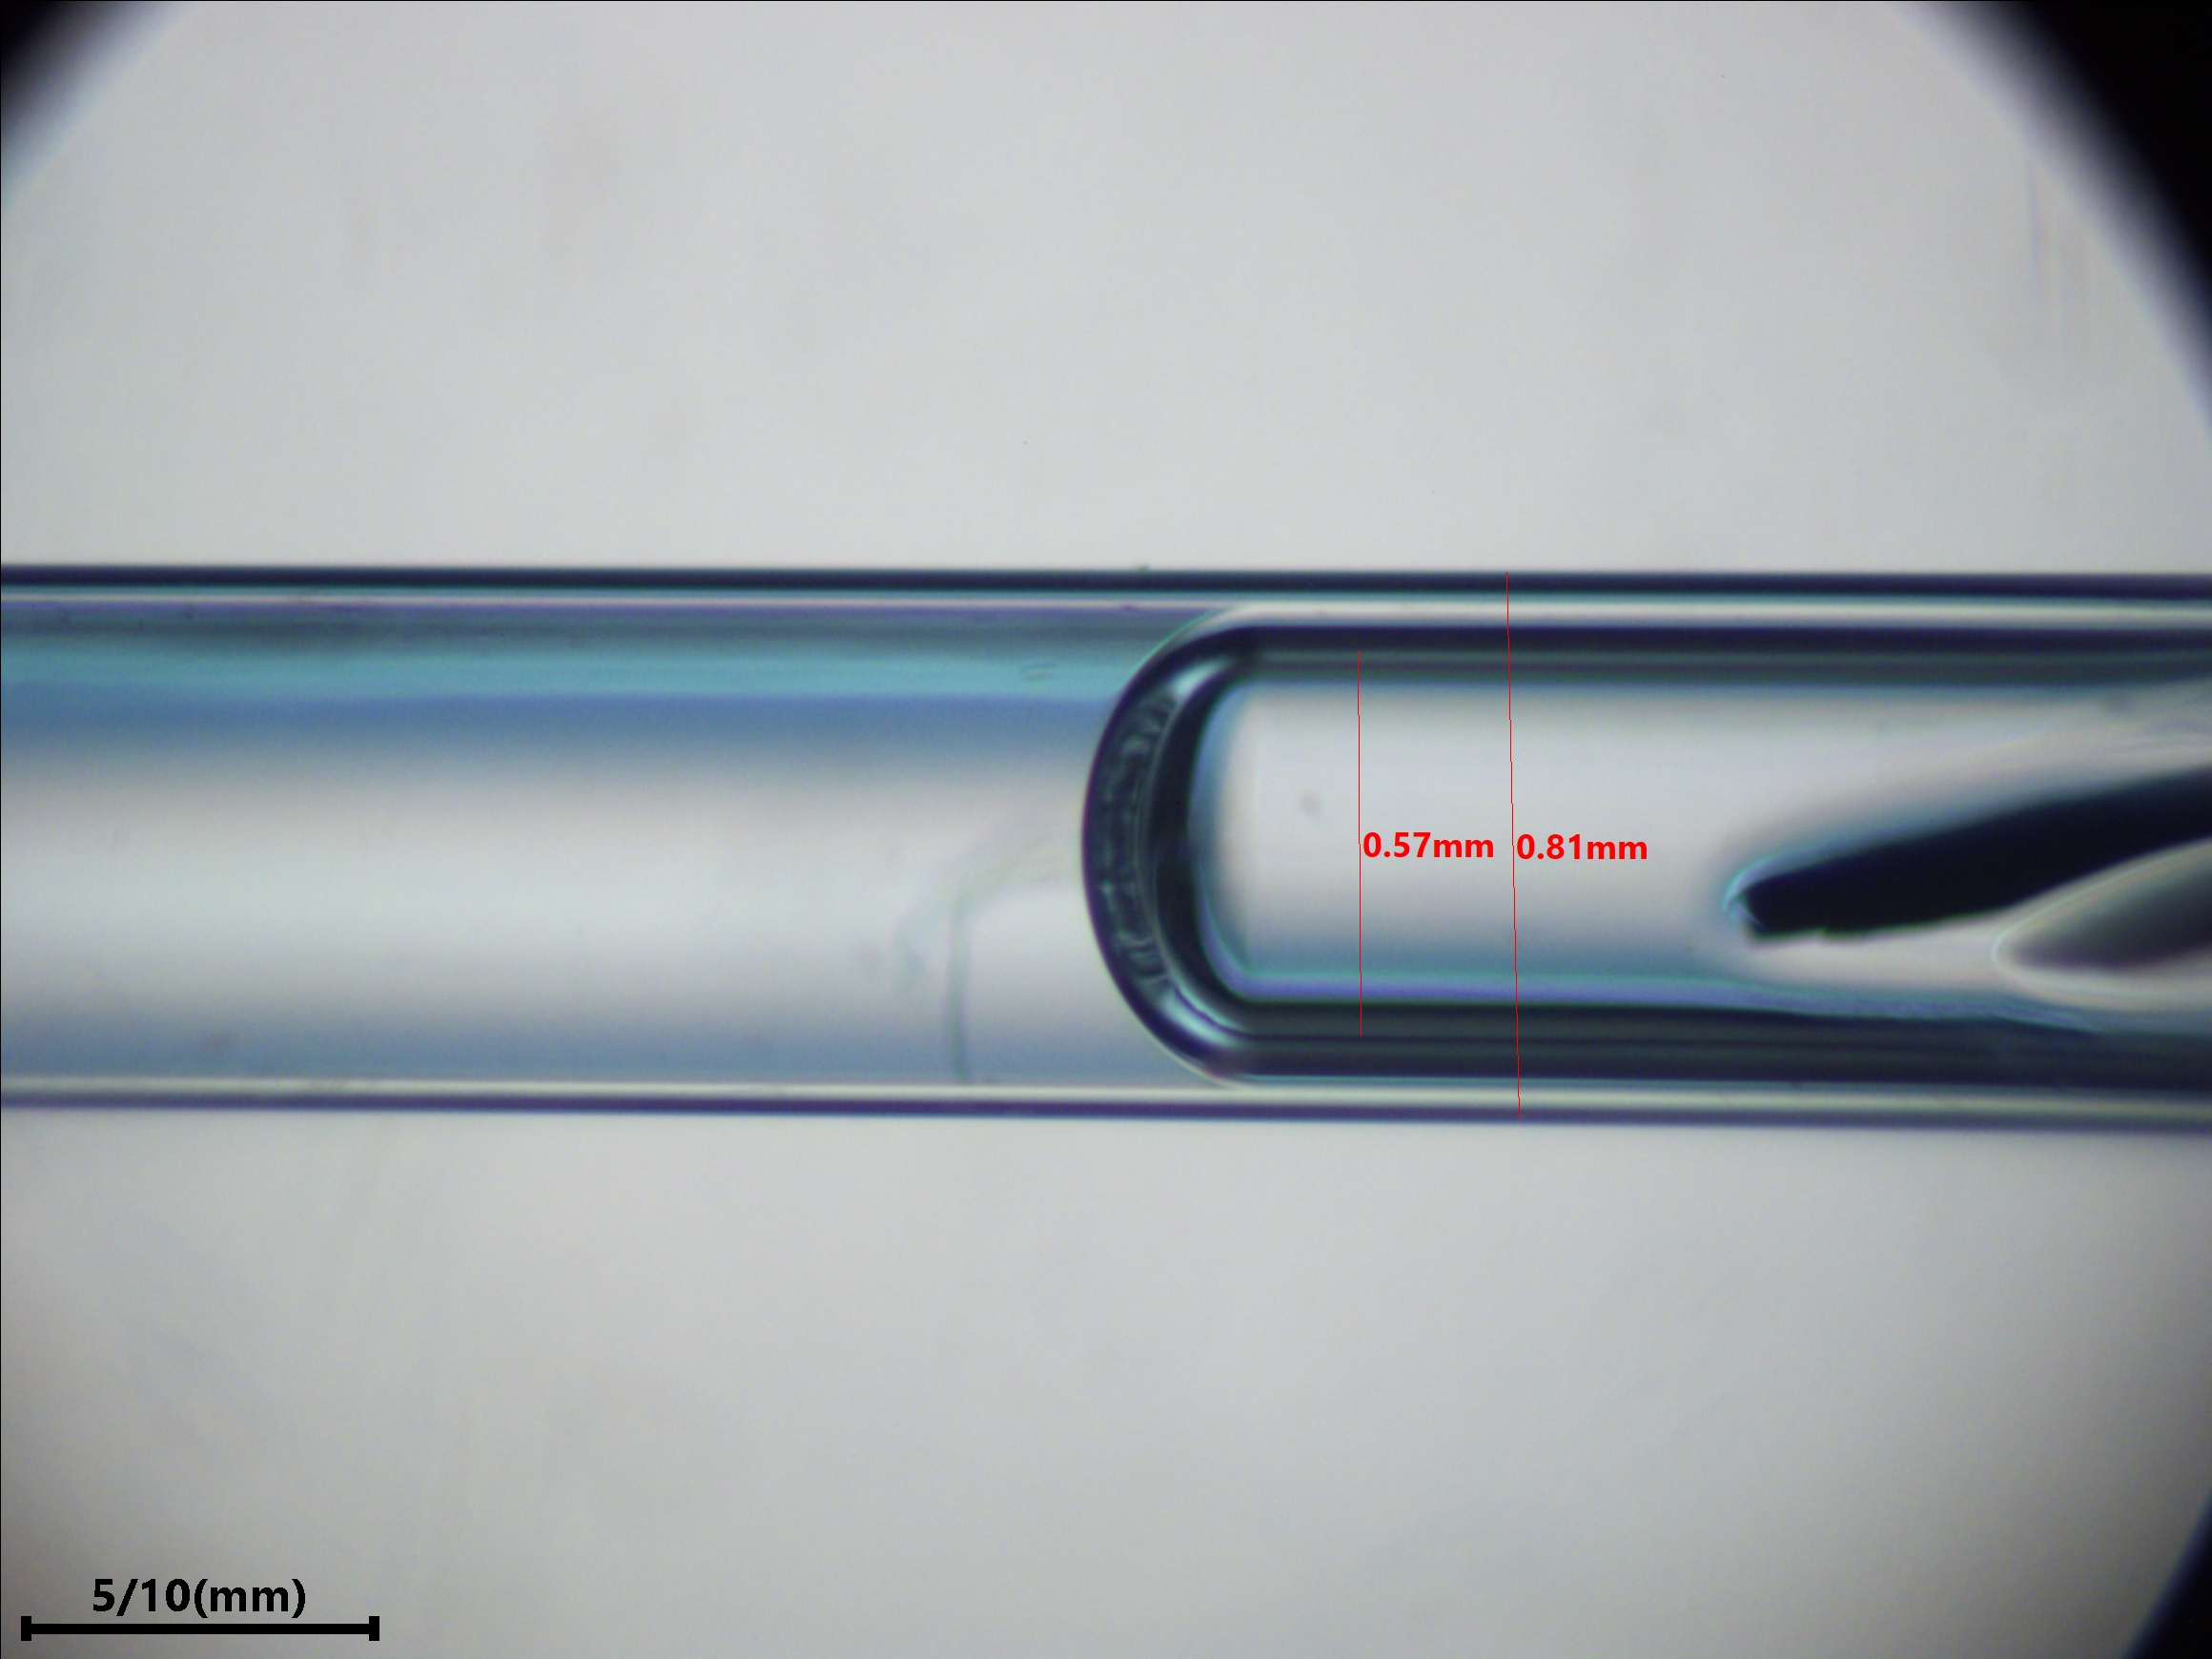
\includegraphics[width=0.7\textwidth]{measureGoeTube.jpg}
\caption{Measurements of the inner and outer diameter of the ampoule used in the water vapor saturated step heats of Win-06-01b. The inner walls of the ampoule are only clearly visible within air bubbles.}
\label{fig:ch2-ampoule-dims}
\end{figure}

\begin{figure}[htbp]
\centering
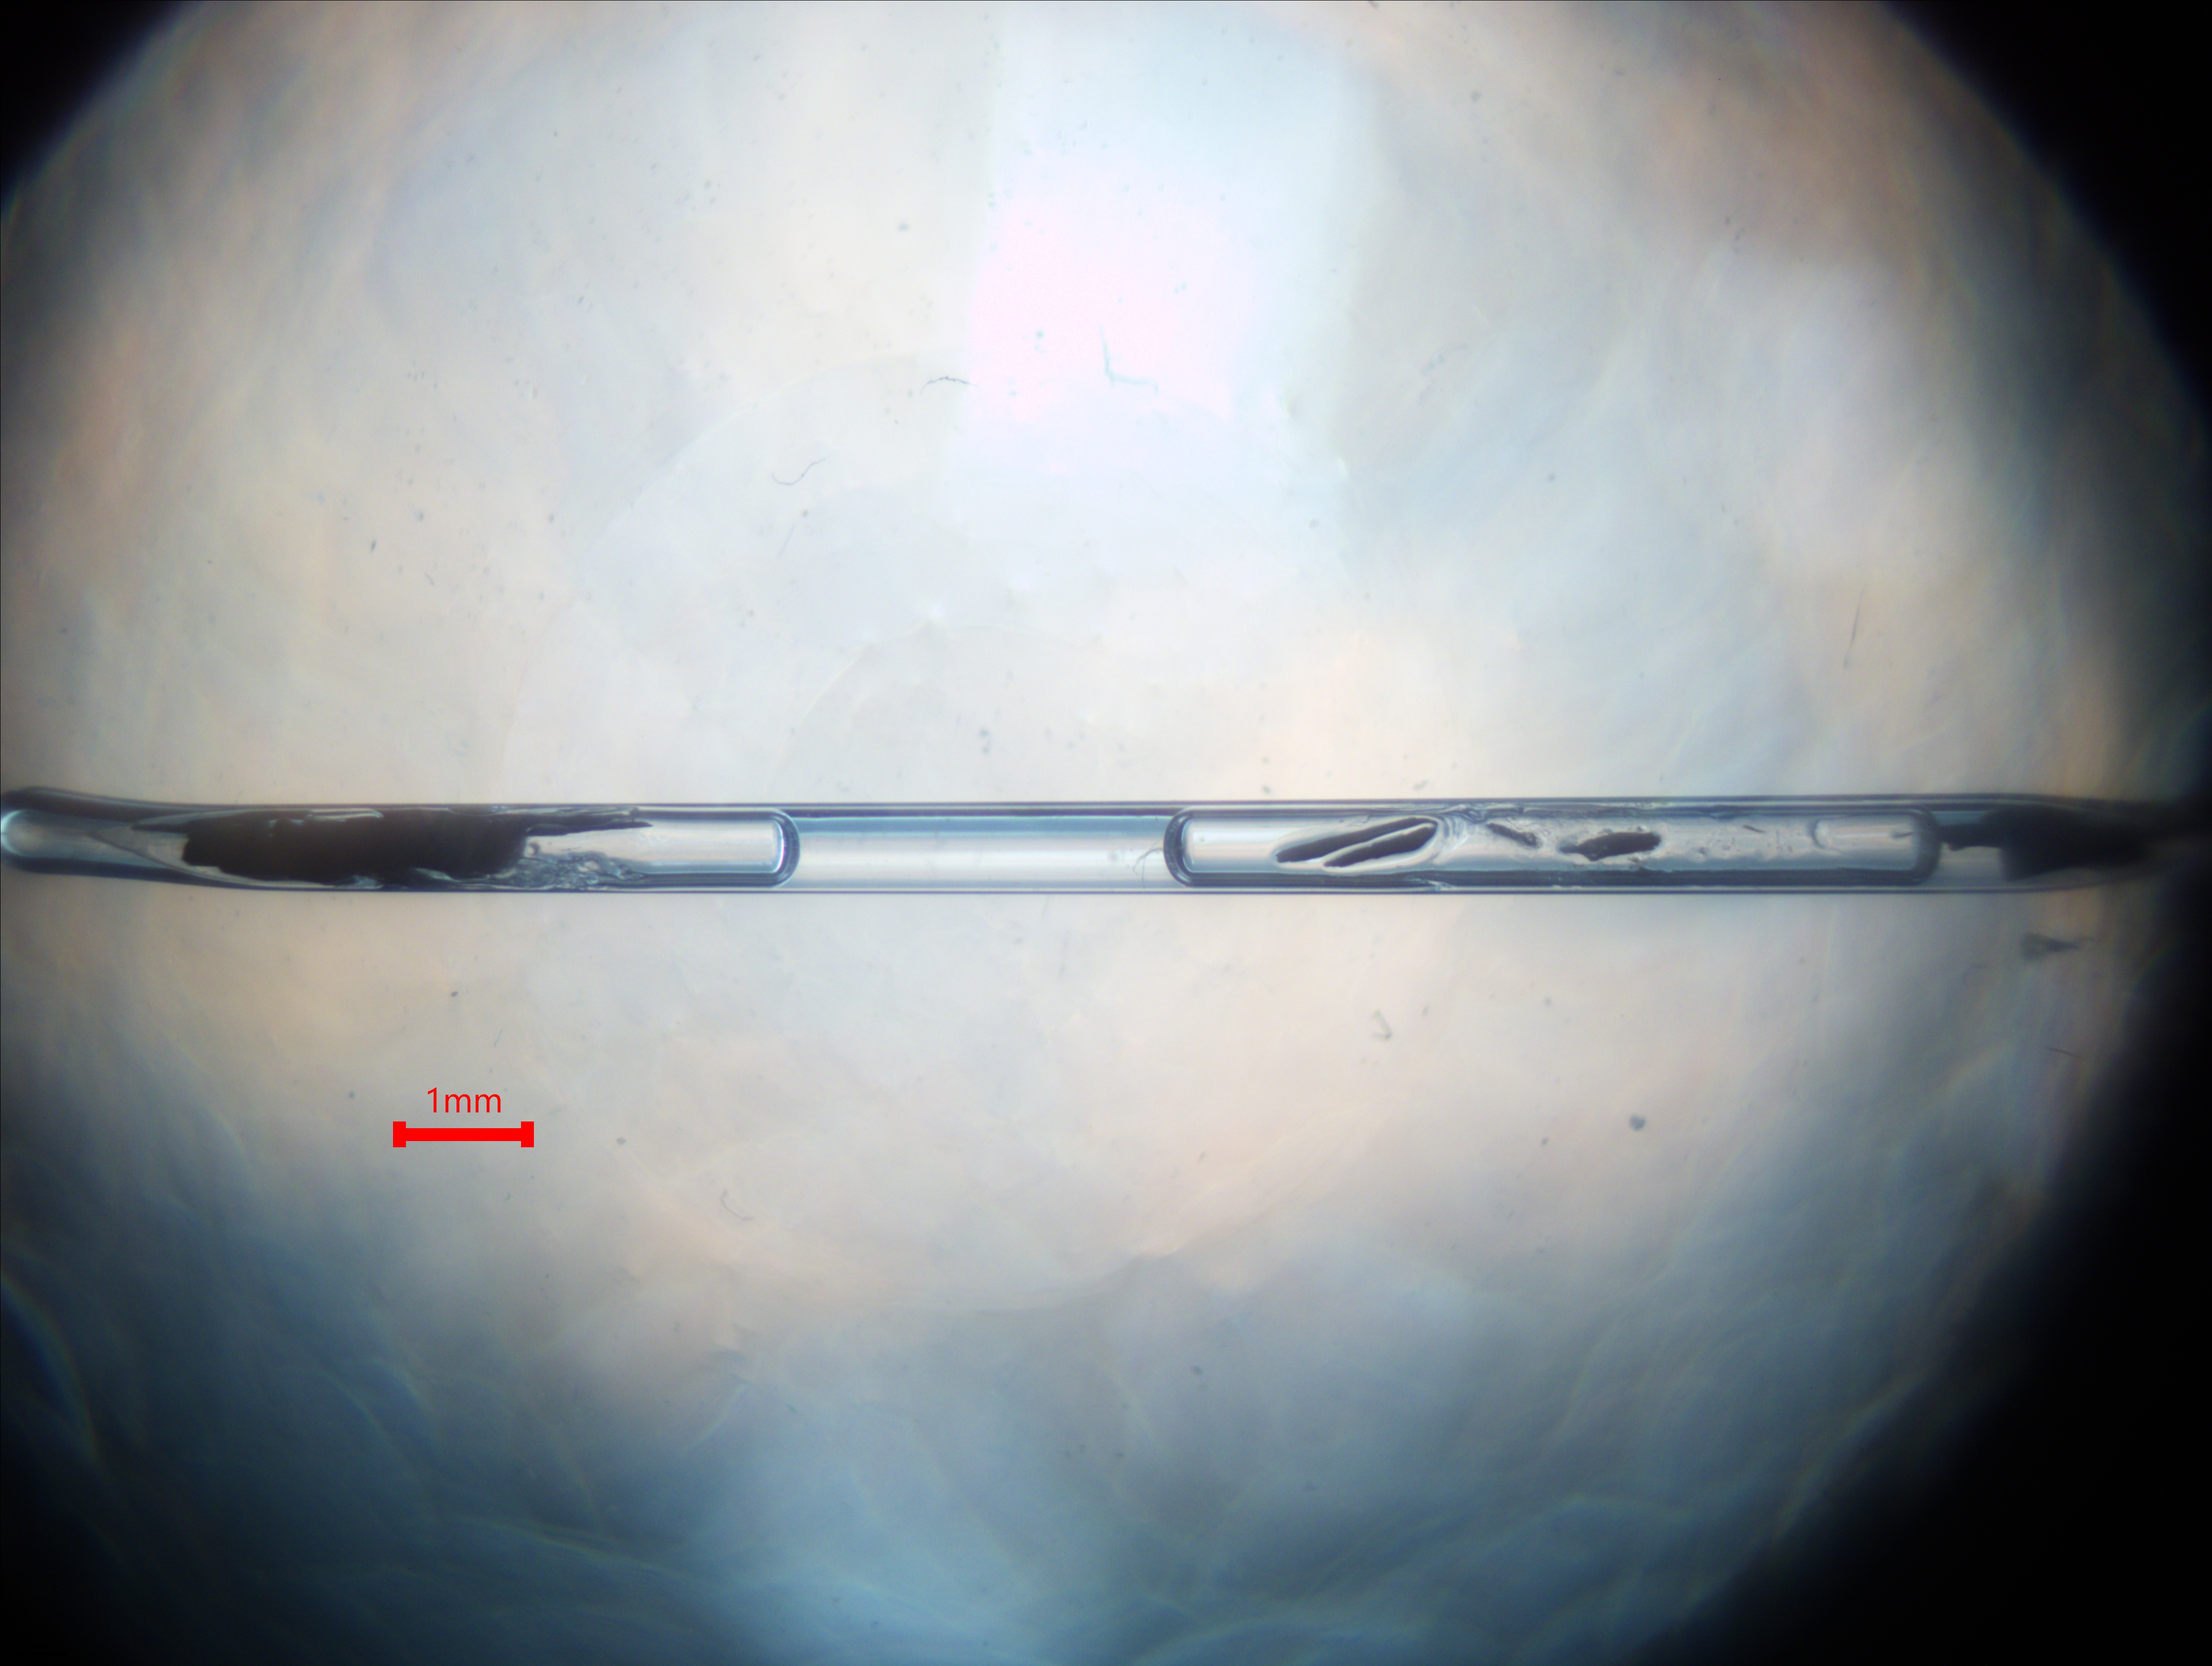
\includegraphics[width=0.7\textwidth]{zoomout2.jpg}
\caption{A view of the entire experimental ampoule after the completion of the step heat experiment before it was broken for the final step in the resistance furnace. At room temperature, the tube is approximately half-filled with gas, one-third filled with liquid water, and one-sixth filled with $<$2\,mm long shards of irradiated Win-06-01b goethite. A gel-like substance was observed lining the inner walls of the tube, which is likely to be amorphous silica dissolved from the tube and redeposited by the thermally-cycled, high pressure liquid water phase.}
\label{fig:ch2-ampoule-post}
\end{figure}

\section{Analytical Methods}\label{ch2-analytical-methods}

\subsection{Final Step}\label{sec:ch2-si-finalstep}

A
hot furnace blank subjected to the same volume splits as the final
HT-Win-06-01b measurement gave a \textsuperscript{3}He blank of 6.8 fccSTP and a \textsuperscript{4}He blank
of 0.31 nccSTP. This blank correction was less than 1\% of the measured
\textsuperscript{4}He and negligible for \textsuperscript{3}He. A re-extract of HT-Win-06-01b immediately
following the measurement yielded above-blank \textsuperscript{3}He and \textsuperscript{4}He signals, which
were added to the total measurement, although both constituted less than
1\% of the final step yield. Sensitivity was calculated by measuring a
\textsuperscript{3}He-enriched air standard with known \textsuperscript{3}He and \textsuperscript{4}He contents immediately
before the measurement.

\section{Kinetic mechanisms and the limits of a single heating schedule}
\label{sec:gt_supp_mech}

Solid-state rate laws separate the temperature dependence of the rate from its dependence on
the extent of reaction \citep{vyazovkin2011}:
\begin{equation}
  \frac{d\alpha}{dt} = A\exp\!\left(-\frac{E_a}{RT}\right)h(\alpha),
\end{equation}
where $\alpha$ is the fraction of goethite converted. The reaction model $h(\alpha)$ expresses the
mechanism: it describes how the rate changes as conversion proceeds, which depends on where
and how the reaction advances through a grain. For first-order kinetics (F1), grains convert
independently once nucleated, so the rate is proportional to the goethite remaining,
$h = 1-\alpha$. For a reaction front moving inward from the grain surface (R2, R3), the rate is
proportional to the shrinking area of the unreacted core. For random nucleation followed by growth
(A2, A3), the rate first accelerates and then slows. For any heating schedule, each rate law
gives $\alpha$ as a function of a single variable,
\begin{equation}
  x = A\sum_j \Delta t_j\exp\!\left(-\frac{E_a}{RT_j}\right),
\end{equation}
the Arrhenius-weighted time delivered by the steps up to the current one; for a single isothermal
step, $x = kt$. We tested the mechanisms in Table~\ref{tab:gt_mech_forms}, including spherical
diffusion on the same footing: for diffusion, $x$ is the Fourier number $Dt/a^2$ with $D/a^2$
Arrhenius in $T$. Under vacuum, the driving-force factor $1-\exp(-\Delta\mu/RT)$ is unity to better
than $10^{-9}$, so $x$ depends only on the heating schedule. Diffusion and conversion then differ
only in the shape of $\alpha(x)$ and in the fitted $E_a$.

\begin{table}[htbp]
  \centering
  \caption{Kinetic models: reaction model $h(\alpha)$ and conversion as a function of the Arrhenius-weighted time, $\alpha(x)$.}
  \label{tab:gt_mech_forms}
  \footnotesize
  \setlength{\tabcolsep}{4pt}
  \begin{tabular}{lll}
    \hline
    Model & $h(\alpha)$ & $\alpha(x)$ \\
    \hline
    R2 contracting cylinder & $2(1-\alpha)^{1/2}$ & $1-(1-x)^2$ \\
    R3 contracting sphere & $3(1-\alpha)^{2/3}$ & $1-(1-x)^3$ \\
    F1 first order & $1-\alpha$ & $1-e^{-x}$ \\
    A2, A3 Avrami ($n=2,3$) & $n(1-\alpha)[-\ln(1-\alpha)]^{1-1/n}$ & $1-e^{-x^n}$ \\
    D3 sphere diffusion & --- & $1-\dfrac{6}{\pi^2}\displaystyle\sum_{m=1}^{\infty} \dfrac{e^{-m^2\pi^2 x}}{m^2}$ \\
    \hline
  \end{tabular}
\end{table}

\subsection{Fits to the vacuum data} Table~\ref{tab:gt_mech_fits} gives the fit of each model to
the cumulative KAF $^3$He release within the fitting window. It also gives the misfit of the
resulting out-of-sample prediction of HDM, and the fit to the KAF water data. F1 gives the best
fit and the best prediction. R3 and R2 are close behind, so we describe the mechanism as
nucleation- or interface-controlled rather than claim first order specifically. The Avrami
fits reach the lower bound of $E_a$ and fail on both data sets. Spherical diffusion with
$\phi=0$ fits KAF \ChTwoKinDThreeRmsRatio{} times worse than F1 and cannot produce the $F\approx0.89$
plateau. To compare diffusion on the same footing, we also fit D3 with $\phi$ fixed at the F1 value
and with $\phi$ free, over the same \ChTwoKinNKAF{} KAF steps. The imposed plateau improves the KAF
misfit to \ChTwoKinDThreePhiRmsKAF{} and \ChTwoKinDThreeFreeRmsKAF, which still ranks below F1, R3 and
R2, and the out-of-sample prediction of HDM does not improve (rms \ChTwoKinDThreePhiRmsHDM{} and
\ChTwoKinDThreeFreeRmsHDM, against \ChTwoKinFOneRmsHDM{} for F1). These fits also require
$E_a$ of \ChTwoKinDThreePhiEa--\ChTwoKinDThreeFreeEa~kJ\,mol$^{-1}$ and a rate factor
$s = \ChTwoKinDThreePhiS$ for the trap-isolated steps, although a diffusive process should not
respond to the water pressure at all.

The fitting window excludes the low-temperature steps, where release is dominated by diffusion from
goethite, and the plateau, where it is dominated by diffusion from hematite; the rms misfits are
computed over the same steps. Repeating the fits with every step included gives the same result:
F1 remains the best model ($E_a = \ChTwoKinAllFOneEa$~kJ\,mol$^{-1}$, $\phi = \ChTwoKinAllPhi$, rms \ChTwoKinAllFOneRmsKAF{} for KAF and \ChTwoKinAllFOneRmsHDM{}
for the HDM prediction), followed by R3 (\ChTwoKinAllRThreeEa~kJ\,mol$^{-1}$; \ChTwoKinAllRThreeRmsKAF, \ChTwoKinAllRThreeRmsHDM) and R2 (\ChTwoKinAllRTwoEa~kJ\,mol$^{-1}$;
\ChTwoKinAllRTwoRmsKAF, \ChTwoKinAllRTwoRmsHDM), with D3 at \ChTwoKinAllDThreeEa~kJ\,mol$^{-1}$ (\ChTwoKinAllDThreeRmsKAF, \ChTwoKinAllDThreeRmsHDM;
\ChTwoKinAllDThreePhiRmsKAF{} and \ChTwoKinAllDThreePhiRmsHDM{} with $\phi$ fixed at the F1 value).

\begin{table}[htbp]
  \centering
  \caption{Kinetic and Diffusive Model fits to the vacuum experiments (from \citet{monteiro2017}~and~\citet{farley2024}). $s$: rate factor for the trap-isolated steps. All rms values are over the same \ChTwoKinNKAF{} KAF and \ChTwoKinNHDM{} HDM steps. D3 is fitted with $\phi$ fixed at 0, fixed at the F1 value, and free; the water fit does not depend on $\phi$ and is given once.}
  \label{tab:gt_mech_fits}
  \begin{tabular}{lccccccc}
    \hline
    Model & $E_a$ & $\ln A$ & $\phi$ & $s$ & rms KAF & rms HDM & $E_a$ (water) \\
    \hline
\ChTwoKinMechFitRows
    \hline
    \multicolumn{8}{l}{\footnotesize $E_a$ in kJ\,mol$^{-1}$, $A$ in s$^{-1}$. $^{a}$At the lower bound of the fit.}
  \end{tabular}
\end{table}

\section{Thermodynamics of Goethite Dehydroxylation}
\label{sec:eqm-thermo}\label{sec:gt_thermo}

Goethite breaks down to hematite by the dehydroxylation reaction
\begin{equation}
  2\,\alpha\text{-FeOOH} \;\rightleftharpoons\; \alpha\text{-Fe}_2\text{O}_3 + \text{H}_2\text{O}_{(\text{fluid})},
  \label{eq:gt_rxn}
\end{equation}
whose Gibbs energy change, written per mole of hematite formed, is
\begin{equation}
  \Delta G_r(T,P) = G_{\mathrm{hem}}(T,P) + G_{\mathrm{w}}(T,P) - 2\,G_{\mathrm{goe}}(T,P) + \Delta G_{\mathrm{surf}} .
  \label{eq:gt_dGr}
\end{equation}
where $\Delta G_r$ is the Gibbs energy change of the reaction and $G_{\mathrm{hem}}$, $G_{\mathrm{w}}$, and $G_{\mathrm{goe}}$ are the Gibbs energies of hematite, water, and goethite, respectively. 
$\Delta G_{\mathrm{surf}}$ is the surface energy contribution, which must be considered to reproduce observed phase stability \citep{navrotsky2008}. 
Goethite is stable where $\Delta G_r>0$ and hematite plus water where $\Delta G_r<0$. The values and equations used to evaluate each of these terms are given below.

\textit{Gibbs energies of the solids.} The Gibbs energy of a phase at $(T,P)$ follows from
integrating $dG = -S\,dT + V\,dP$ from the reference state $(T_r,P_r) = (298.15~\mathrm{K}, 1~\mathrm{bar})$,
first in temperature at $P_r$ and then in pressure at $T$. At $P_r$,
$H(T) = H(T_r) + \int_{T_r}^{T}C_p\,dT$ and $S(T) = S(T_r) + \int_{T_r}^{T}(C_p/T)\,dT$, so
$G(T,P_r) = H(T) - T S(T)$. Adding $\int_{P_r}^{P}V\,dP$, and treating the solids as incompressible
with no thermal expansion, gives
\begin{equation}
  G_i(T,P) = \Delta_f H_i^{0} + \int_{T_r}^{T} C_{p,i}\,dT
  \;-\; T\left[S_i^{0} + \int_{T_r}^{T}\frac{C_{p,i}}{T}\,dT\right]
  \;+\; V_i\,(P-P_r),
  \label{eq:gt_Gsolid}
\end{equation}
where $H(T_r) = \Delta_f H_i^{0}$ and $S(T_r) = S_i^{0}$. This is the ``apparent'' Gibbs energy of
formation \citep{berman1988}; the element-entropy terms that distinguish it from the true Gibbs
energy of formation cancel in any balanced reaction. Compressibility and thermal expansion change
$V_i$ by $\lesssim1\%$ over the conditions considered and are neglected.

Goethite heat capacity uses the Berman--Brown form \citep{berman1985} refined by
\citet{majzlan2003}, $C_p = k_0 + k_1 T^{-1/2} + k_2 T^{-2} + k_3 T^{-3}$. Hematite uses the same
polynomial with the coefficients of \citet{berman1988}, which \citet{majzlan2003} held fixed in their
refinement. Both heat capacities are integrated analytically.

\textit{Water.} Water is evaluated with the IAPWS-95 equation of state \citep{wagner2002},
implemented in CoolProp \citep{bell2014}, which is valid for liquid, vapor and supercritical
water to 1~GPa. In the same apparent convention,
\begin{equation}
  G_{\mathrm{w}}(T,P) = \Delta_f H_{\mathrm{w}}^{0} + \left[h(T,P) - h(T_r,P_r)\right]
  - T\left[S_{\mathrm{w}}^{0} + s(T,P) - s(T_r,P_r)\right],
  \label{eq:gt_Gw}
\end{equation}
where $h$ and $s$ are the IAPWS-95 molar enthalpy and entropy and the reference state is liquid
water at $T_r,P_r$. Table~\ref{tab:gt_thermo_data} lists all
input data. We use the enthalpies and entropies of \citet{majzlan2003} refined by mathematical
programming against the phase-equilibrium brackets of \citet{voigt1981}.

\begin{table}[htbp]
  \centering
  \caption{Thermodynamic data used for Eq.~\eqref{eq:gt_dGr}.}
  \label{tab:gt_thermo_data}
  \begin{footnotesize}
  \begin{tabular}{lcc}
    \hline
    & Goethite ($\alpha$-FeOOH) & Hematite ($\alpha$-Fe$_2$O$_3$) \\
    \hline
    $\Delta_f H^0$ (kJ\,mol$^{-1}$) & $-561.4$ & $-825.8$ \\
    $S^0$ (J\,mol$^{-1}$\,K$^{-1}$) & 59.5 & 87.4 \\
    $V^0$ (cm$^3$\,mol$^{-1}$) & 20.881 & 30.274 \\
    $C_p$ coefficients & $k_0=133.8765$ & $k_0=146.86$ \\
          & $k_1=-738.5577$ & $k_1=0$ \\
          & $k_2=-2.177657\times10^{6}$ & $k_2=-5.5768\times10^{6}$ \\
          & $k_3=2.165124\times10^{8}$ & $k_3=5.2563\times10^{8}$ \\
    $C_p(298\ \mathrm{K})$ (J\,mol$^{-1}$\,K$^{-1}$) & 74.8 & 104.0 \\
    $\gamma_{\mathrm{hydrated}}$ (J\,m$^{-2}$) & $0.60\pm0.10$ & $0.75\pm0.16$ \\
    $\gamma_{\mathrm{anhydrous}}$ (J\,m$^{-2}$) & $0.91\pm0.09$ & $1.90\pm0.30$ \\
    \hline
  \end{tabular}
  \end{footnotesize}

  \vspace{0.5ex}
  \begin{minipage}{0.85\linewidth}\footnotesize
  Enthalpy and entropy: \citet{majzlan2003}; goethite $C_p$: \citet{majzlan2003a,majzlan2003};
  hematite $C_p$: \citet{berman1988}; surface energies: \citet{navrotsky2008}.
  Units: $k_0$ J\,mol$^{-1}$\,K$^{-1}$, $k_1$ J\,mol$^{-1}$\,K$^{-1/2}$, $k_2$ J\,K\,mol$^{-1}$,
  $k_3$ J\,K$^{2}$\,mol$^{-1}$; $l_1$ (J\,mol$^{-1}$)$^{1/2}$\,K$^{-1}$, $l_2$ (J\,mol$^{-1}$)$^{1/2}$\,K$^{-2}$.
  Water: $\Delta_f H^0_{\mathrm{w}} = -285.83$~kJ\,mol$^{-1}$, $S^0_{\mathrm{w}} = 69.95$~J\,mol$^{-1}$\,K$^{-1}$; IAPWS-95 for $h(T,P)$, $s(T,P)$.
  \end{minipage}
\end{table}

As a check, at 298.15~K and 1~bar with liquid water, Eqs.~\eqref{eq:gt_dGr}--\eqref{eq:gt_Gw}
give $\Delta G_r = -0.26$~kJ: hematite plus liquid water is favored by only 0.13~kJ per mole of
FeOOH. This is well inside the $\pm1.4$~kJ\,mol$^{-1}$ uncertainty that \citet{majzlan2003}
assign to the goethite--hematite free-energy difference; the two assemblages are essentially
balanced at ambient conditions. We carry this uncertainty ($\pm2.8$~kJ per reaction as written)
as bounding curves on the phase diagram.

\textit{Surface energy.} A crystal of finite size carries an excess free energy at its
surface in addition to the free energy of its bulk \citep{gibbs1878}. For a population of
particles of fixed size, this excess is $\gamma A$, where $\gamma$ is the surface energy
(J\,m$^{-2}$) and $A$ the total surface area. Both the bulk and surface terms scale with the
amount of material at fixed particle size, so the surface contribution can be written per mole,
$G = G_{\mathrm{bulk}} + \gamma A_m$, with $A_m$ the surface area per mole. $A_m$ grows as $1/d$,
so the term is negligible for coarse crystals and significant for nanoparticles
\citep{navrotsky2008}. For the reaction as written (one mole of hematite from two moles of
goethite),
\begin{equation}
  \Delta G_{\mathrm{surf}} = \gamma_{\mathrm{hem}} A_{m,\mathrm{hem}} - 2\,\gamma_{\mathrm{goe}} A_{m,\mathrm{goe}},
  \label{eq:gt_dGsurf}
\end{equation}
where $A_{m,\mathrm{hem}}$ is per mole of Fe$_2$O$_3$ and $A_{m,\mathrm{goe}}$ per mole of FeOOH.

A size must be chosen for each phase. We assume pseudomorphic dehydroxylation, in which hematite
inherits the external envelope of the parent goethite, so that both phases share the same
external surface area per mole of Fe. This is also the basis of the stability diagrams of
\citet{navrotsky2008}. For spherical goethite grains of diameter $d$ this shared area is
\begin{equation}
  A_{\mathrm{Fe}} = \frac{6\,V_{\mathrm{goe}}}{d}\quad\text{per mole of Fe}.
\end{equation}
Goethite has one Fe per formula unit, so $A_{m,\mathrm{goe}} = A_{\mathrm{Fe}}$. Hematite has two,
so $A_{m,\mathrm{hem}} = 2A_{\mathrm{Fe}}$. Substituting into Eq.~\eqref{eq:gt_dGsurf},
\begin{equation}
  \Delta G_{\mathrm{surf}} = \gamma_{\mathrm{hem}}\,(2A_{\mathrm{Fe}}) - 2\,\gamma_{\mathrm{goe}}\,A_{\mathrm{Fe}}
  = 2A_{\mathrm{Fe}}\left(\gamma_{\mathrm{hem}} - \gamma_{\mathrm{goe}}\right).
  \label{eq:gt_equalarea}
\end{equation}
The factor of two counts the two moles of Fe that pass through the reaction. It multiplies both
terms because both phases carry the same area per Fe. For $d=10$~nm,
$A_{\mathrm{Fe}} = 6\times20.881\times10^{-6}/10^{-8} = 1.253\times10^{4}$~m$^2$\,mol$^{-1}$, and
with hydrated surface energies
$\Delta G_{\mathrm{surf}} = 2\times1.253\times10^{4}\times(0.75-0.60) = +3.76$~kJ.
The corresponding values are $+0.38$~kJ at 100~nm and $+0.04$~kJ at 1~\textmu m. A positive
$\Delta G_{\mathrm{surf}}$ stabilizes goethite. If the two phases are instead compared at equal
particle diameter, the same hydrated surface energies slightly destabilize fine goethite
($-1.41$~kJ at 10~nm). The choice affects only the stability discussion; the kinetic analysis uses
bulk driving forces.

We use hydrated surface energies. They are referenced to liquid water, so they apply wherever the
surfaces are in equilibrium with water at or near saturation, which includes all of the water vapor saturated experiments. Anhydrous surface energies apply only to surfaces that have lost their
chemisorbed water, i.e.\ under vacuum.

\textit{Phase diagram.} The phase diagram (Fig.~\ref{fig:gt_PT}) is computed by solving
$\Delta G_r(T,P) = 0$ (Eqs.~\eqref{eq:gt_dGr}--\eqref{eq:gt_equalarea}) numerically for
$P = P_{\mathrm{H_2O}}$ at each temperature, using Brent's method on $\log_{10}P$ between
$10^{-12}$ and $10^{4}$~bar, with the solids at the fluid pressure. Where no root exists below the
melting curve of ice, the curve is truncated.

\textit{Driving force and the role of water.} The quantity that matters for kinetics is the
driving force for hematite formation, $\Delta\mu \equiv -\Delta G_r/N_A$ (per mole of Fe$_2$O$_3$).
Water controls $\Delta\mu$ through its own chemical potential, because it is a product of
reaction~\eqref{eq:gt_rxn}. $G_{\mathrm{w}}$ in Eq.~\eqref{eq:gt_dGr} is the chemical potential of
H$_2$O at the prevailing water fugacity. It depends on the partial pressure of water, not on the
total pressure. An inert gas, or any other mechanical load, acts only through the solid-volume
term $\Delta V_s(P-P_r)$, which contributes $-1.15$~J\,bar$^{-1}$ and slightly favors the denser
hematite. At 40~bar that is 46~J, three orders of magnitude smaller than the effect of 40~bar of
water. The water-buffered step-heating technique therefore stabilizes goethite primarily by
reducing the driving force of the reaction. Surface hydration is a second-order correction that matters
only for nanometer grains (Eq.~\eqref{eq:gt_equalarea}).

\subsection{Stability and driving force}

The model can be used to calculate the stability field for
goethite with respect to dehydroxylation to hematite and water in $\log P_{\mathrm{H_2O}}$--$T$ space (Fig.~\ref{fig:gt_PT}). This 
phase diagram communicates several important features of the goethite--hematite--water system that are relevant to the experiments considered here:
\begin{enumerate}
  \item Goethite is not stable at the conditions of any of the experiments considered here, in water or in vacuum, in spite of the evidence that it did not react in the water-saturated experiment. Thus, we hypothesize that the reaction is kinetically inhibited for goethite under these conditions.
  \item The stability of goethite is strongly dependent on the partial pressure of water below and up to water saturation. Above the saturation pressure, water is liquid and contributes far less to the reaction volume than it does as a gas, becoming a secondary control on goethite's stability.
  \item The stability of goethite is strongly dependent on grain size, with smaller grains being more stable than larger grains. At water saturation, bulk goethite is stable below 18~$^\circ$C, 100~nm goethite below 28~$^\circ$C, and 10~nm goethite below 108~$^\circ$C. 
\end{enumerate}

\begin{figure}[htbp]
  \centering
  \includegraphics[width=0.7\linewidth]{goethite_hematite_Ph2o_T_hydrated.pdf}
  \caption{Goethite--hematite--water equilibrium in $\log P_{\mathrm{H_2O}}$--$T$ space for bulk
  goethite and for 100 and 10~nm grains with hydrated surfaces, compared at equal surface area
  per mole of Fe (Eq.~\eqref{eq:gt_equalarea}). Goethite is stable above and to the left of each
  curve. The dash-dot curves illustrate the absolute uncertainty: it is the bulk stability boundary shifted by the $\pm1.4$~kJ\,mol$^{-1}$ FeOOH uncertainty of
  \citet{majzlan2003}. The blue dotted curve shows the water vapor saturation pressure; liquid water is present at and above this curve. The thermodynamic data used to compute the phase diagram are in
  Table~\ref{tab:gt_thermo_data}.}
  \label{fig:gt_PT}
\end{figure}

Stability alone does not determine what happens in a step heat; the rate of conversion controls
whether this equilibrium state is reached or if the reaction proceeds at all,
and that depends on the chemical potential of the reaction: $\Delta\mu$. Table~\ref{tab:gt_dmu} gives the bulk driving
forces at the experimental temperatures, evaluated with IAPWS-95 water. At saturation,
$\Delta\mu$ is 6--11~kJ, only 1.6--2.4 times $RT$. Under the vacuum of a step-heating line the water
pressure approaches zero, so the chemical potential of water falls without bound and $\Delta\mu$ is
unbounded. The chemical
potential of water is therefore the key variable separating the two experimental settings.

\begin{table}[htbp]
  \centering
  \caption{Bulk driving force for hematite formation, $\Delta\mu = -\Delta G_r$ (kJ per mole Fe$_2$O$_3$), at water saturation. In vacuum ($P_{\mathrm{H_2O}}\rightarrow0$) the driving force is unbounded.}
  \label{tab:gt_dmu}
  \begin{tabular}{cccc}
    \hline
    $T$ ($^\circ$C) & $P_{\mathrm{sat}}$ (bar) & $\Delta\mu_{\mathrm{sat}}$ & $\Delta\mu_{\mathrm{sat}}/RT$ \\
    \hline
    150 & 4.76  & 5.68  & 1.61 \\
    175 & 8.93  & 6.88  & 1.84 \\
    200 & 15.55 & 8.11  & 2.06 \\
    225 & 25.50 & 9.37  & 2.26 \\
    250 & 39.76 & 10.66 & 2.45 \\
    \hline
  \end{tabular}
\end{table}

\section{Nucleation Model of Goethite Dehydroxylation}\label{sec:gt_nuc_si}

\textit{Nucleation barrier.} In classical nucleation theory \citep{gibbs1878,volmer1926,becker1935},
reviewed by \citet{christian2002}, \citet{kashchiev2000} and, for mineral systems,
\citet{deyoreo2003} and \citet{lasaga1998}, a spherical hematite nucleus of radius $r$ has free
energy
\begin{equation}
  \Delta G(r) = -\frac{4}{3}\pi r^{3}\,\frac{\Delta\mu}{V_{\mathrm{hem}}} + 4\pi r^{2}\gamma,
\end{equation}
where $\Delta\mu$ is the driving force per mole of Fe$_2$O$_3$ (Table~\ref{tab:gt_dmu}),
$V_{\mathrm{hem}}$ the molar volume and $\gamma$ the energy of the interface surrounding the
nucleus. Nuclei larger than the critical radius $r^{*} = 2\gamma V_{\mathrm{hem}}/\Delta\mu$ grow,
and the energetic barrier to forming one is
\begin{equation}
  \Delta G^{*} = \frac{16\pi\,\gamma^{3}\,V_{\mathrm{hem}}^{2}}{3\,\Delta\mu^{2}} .
  \label{eq:gt_barrier}
\end{equation}
In the first-order limit of \S\ref{sec:gt_vacuum}, the rate constant is a nucleation rate of the
form derived by \citet{turnbull1949},
\begin{gather}
  k = A\exp\!\left(-\frac{E_a}{RT}\right)\exp\!\left(-\frac{\Delta G^{*}}{k_B T}\right), \notag\\
  \frac{\Delta G^{*}}{k_B T} = \frac{C\gamma^{3}}{T\,\Delta\mu^{2}},
  \qquad
  C \equiv \frac{16\pi V_{\mathrm{hem}}^{2}}{3k_B} = 1.112\times10^{15}~\mathrm{m^6\,K\,J^{-1}\,mol^{-2}} ,
  \label{eq:gt_knuc}
\end{gather}
where $A\exp(-E_a/RT)$ describes the atomic mobility and $\exp(-\Delta G^{*}/k_BT)$ is the
equilibrium fraction of sites occupied by critical nuclei. Because the barrier scales as
$\gamma^3/\Delta\mu^2$, it vanishes in vacuum, where the water pressure approaches zero and $\Delta\mu$
grows without bound, but is significant at water saturation, where $\Delta\mu$ is only 6--11~kJ
(Table~\ref{tab:gt_dmu}).

\textit{Internal nucleation.} Goethite dehydroxylates topotactically: hematite nucleates within
the parent crystal, inherits its oxygen framework and orientation, and the pseudomorph develops
pores and twinned hematite domains \citep{limadefaria1963,watari1979,watari1983,cudennec2005}.
We therefore consider only internal nucleation, in which the new interface of the burgeoning nuclei is between hematite
and goethite. We know of no measured or calculated energy for that interface, so $\gamma$ is
replaced by an effective parameter $\gamma_{\mathrm{eff}}$, calibrated from the data.

\textit{Calibration.} When \citet{farley2024} isolated the liquid nitrogen trap from the heated goethite, they raised $P_{\mathrm{H_2O}}$ in the line and lowered
$\Delta\mu$, and the isothermal rate fell by a factor $s$ (\S\ref{sec:gt_vacuum}). With $A$ and $E_a$
unchanged, Eq.~\eqref{eq:gt_knuc} gives
\begin{equation}
  \gamma_{\mathrm{eff}} = \left[\frac{T\,\Delta\mu_{\mathrm{off}}^{2}\ln(1/s)}{C}\right]^{1/3},
  \label{eq:gt_gamma_cal}
\end{equation}
where $\Delta\mu_{\mathrm{off}}$ is evaluated at an upper bound on the water pressure with the trap isolated.
This pressure estimate of the water released depends on the
volume of the experimental apparatus and the water content emitted by the goethite, which was measured with 
capacitance manometry (\S\ref{sec:gt_supp_barrier}). With the trap in place, the water pressure approaches zero,
the driving force is unbounded, and its contribution to the barrier vanishes. Any finite water pressure in
the trapped line would give a larger $\gamma_{\mathrm{eff}}$, so this limit is conservative. This gives $\gamma_{\mathrm{eff}} = \ChTwoKinMCGammaMid$~J\,m$^{-2}$
(range \ChTwoKinGammaLo--\ChTwoKinGammaHi). In vacuum the barrier vanishes, so conversion is barrierless,
consistent with the simple Arrhenius behavior of both vacuum experiments. At saturation and
250~$^\circ$C, the critical nucleus has a radius of \ChTwoKinRstarSat~nm (\ChTwoKinNfuSat{} formula units)
and the barrier is \ChTwoKinBarSat~$k_BT$. For nuclei this small, classical nucleation theory has no
literal meaning, so $\gamma_{\mathrm{eff}}$ is best read as the single parameter of a rate law in which
$\ln k$ falls as $-1/\Delta\mu^{2}$, not as an interface energy.

\textit{Translation to water saturation.} For the same sample, only $\Delta\mu$ changes between
vacuum and saturation:
\begin{equation}
  \frac{k_{\mathrm{sat}}}{k_{\mathrm{vac}}} = \exp\!\left[-\frac{C\gamma_{\mathrm{eff}}^{3}}{T}\frac{1}{\Delta\mu_{\mathrm{sat}}^{2}}\right].
  \label{eq:gt_translate}
\end{equation}
Applied step by step to the water vapor saturated schedule, Eq.~\eqref{eq:gt_translate} predicts a total
conversion ($\sum_i \frac{k_{\mathrm{sat}}}{k_{\mathrm{vac}}}(T_i)\,k_{\mathrm{vac}}(T_i)\,\Delta t_i$) 
of $10^{\ChTwoKinLogAlphaLow}$, $10^{\ChTwoKinLogAlphaMid}$ and $10^{\ChTwoKinLogAlphaHigh}$ for
$\gamma_{\mathrm{eff}} = 0.12$, 0.14 and 0.15~J\,m$^{-2}$, and $10^{\ChTwoKinMCCNTLo}$ to
$10^{\ChTwoKinMCCNTHi}$ (95\%) when the uncertainties in the calibration and in the thermodynamic
data are propagated (\S\ref{sec:gt_supp_barrier}). The exact values reflect the assumed
$\Delta\mu^{-2}$ dependence; what matters is that the model predicts
suppression far beyond the $10^{\ChTwoKinLogRDetect}$ that the data require (main text,
\S\ref{sec:gt_nucleation}).

\textit{Assumptions.} This is a consistent physical explanation of the data, not a proof. It is not exhaustive. This analysis
assumes (i) that the trap-isolated slowdown acts through $\Delta\mu$, rather than, for example,
through water blocking reactive sites; (ii) that $\gamma_{\mathrm{eff}}$, $A$ and $E_a$ are the same in
vacuum and in water; (iii) that the barrier depends on the bulk driving force without significant contribution from surface
terms (this analysis extended to 10~nm grains raises the predicted conversion only to $\sim10^{-13}$;
\S\ref{sec:gt_supp_barrier}); and (iv) that conversion is solid-state. Conversion by dissolution
of goethite and precipitation of hematite from the fluid is not described by
Eq.~\eqref{eq:gt_translate} (see \S\ref{sec:gt_pigment}). The calibrated $\gamma_{\mathrm{eff}}$ absorbs contributions from the
sample's microstructure and cannot be transferred to other goethites.

\subsection{Calibration of $\gamma_{\mathrm{eff}}$}
\label{sec:gt_supp_barrier}

Equation~\eqref{eq:gt_gamma_cal} follows from Eq.~\eqref{eq:gt_knuc} applied to a trap-isolated step
and its trapped neighbors,
$\ln(1/s) = C\gamma_{\mathrm{eff}}^{3}/(T\,\Delta\mu_{\mathrm{off}}^{2})$; the corresponding term for the
trapped neighbors vanishes because their driving force is unbounded (item 2).
The driving forces are evaluated as follows.
\begin{enumerate}
  \item $\Delta\mu_{\mathrm{off}}$ is a bulk driving force,
  $-\Delta G_r$ from Eq.~\eqref{eq:gt_dGr} (\S\ref{sec:eqm-thermo}) with $\Delta G_{\mathrm{surf}} = 0$, at the
  step temperature and with the solids at vacuum.
  \item With the trap in place, the water pressure in the line approaches zero, so the chemical
  potential of water falls without bound, $\Delta\mu_{\mathrm{on}}$ is unbounded, and its term
  $\Delta\mu_{\mathrm{on}}^{-2}$ vanishes. This is the conservative limit: any finite water pressure in
  the trapped line would give a larger $\gamma_{\mathrm{eff}}$ and a stronger predicted slowdown at
  saturation. $\Delta\mu_{\mathrm{off}}$ is evaluated at the water pressure reached with the trap
  isolated (below).
  \item Surface terms are omitted. The barrier of an internal nucleus depends on the free
  energy per volume of material transformed, not on the external surface of the host grain. The external surface
  energy of the grain enters the overall thermodynamic stability (\S\ref{sec:gt_thermo}), but is not
  a part of the nucleation barrier, which is evaluated for internal nuclei.
\end{enumerate}
We bound the water pressure with the trap isolated by assuming that all evolved water was in the
vapor, distributed uniformly through an apparatus of volume $V_{\mathrm{app}}$ at 298~K:
\begin{equation}
  P_{\mathrm{H_2O}} = \frac{(m_{\mathrm{w}}/M_{\mathrm{w}})\,RT}{V_{\mathrm{app}}} .
\end{equation}
With $m_{\mathrm{w}} = 0.027$~mg at 230~$^\circ$C and 0.016~mg at 240~$^\circ$C ($1.50$ and
$0.89~\mu$mol), and $190\le V_{\mathrm{app}}\le600$~mL, Table~\ref{tab:gt_gamma} gives the pressures
and the resulting $\gamma_{\mathrm{eff}}$. The pressures are end-of-step values; we also evaluate half
of each as a time average for steady accumulation. This is an upper bound on the pressure, because
some water adsorbs on the walls of the line; a lower true pressure gives a larger
$\gamma_{\mathrm{eff}}$ and more suppression at saturation, so the bound is conservative. Pressure
enters only through $\ln P$ in $\Delta\mu_{\mathrm{off}}$ and then through $\Delta\mu_{\mathrm{off}}^{2/3}$, so a
threefold uncertainty in volume changes $\gamma_{\mathrm{eff}}$ by only about 5\%. The two steps agree within
20\%, and we adopt $\gamma_{\mathrm{eff}} = \ChTwoKinMCGammaMid$~J\,m$^{-2}$, with a range of
\ChTwoKinGammaLo--\ChTwoKinGammaHi~J\,m$^{-2}$.

\begin{table}[htbp]
  \centering
  \caption{Water pressure with the trap isolated and the calibrated $\gamma_{\mathrm{eff}}$ (J\,m$^{-2}$; Eq.~\eqref{eq:gt_gamma_cal}).}
  \label{tab:gt_gamma}
  \begin{tabular}{cccccc}
    \hline
    $T$ ($^\circ$C) & $s$ & $V_{\mathrm{app}}$ (mL) & $P_{\mathrm{H_2O}}$ (Pa) & $\gamma_{\mathrm{eff}}$, end-of-step $P$ & $\gamma_{\mathrm{eff}}$, $P/2$ \\
    \hline
    230 & 0.333 & 190 & 19.6 & 0.120 & 0.124 \\
    230 & 0.333 & 600 & 6.2  & 0.126 & 0.130 \\
    240 & 0.224 & 190 & 11.6 & 0.140 & 0.145 \\
    240 & 0.224 & 600 & 3.7  & 0.147 & 0.152 \\
    \hline
  \end{tabular}
\end{table}

\subsection{Uncertainty propagation} The Monte Carlo range quoted in \S\ref{sec:gt_nucleation}
(\ChTwoKinNMC{} draws) samples the trap-isolated step (230 or 240~$^\circ$C); $s$, log-uniformly between
\ChTwoKinSLowRange{} at 230~$^\circ$C and \ChTwoKinSHighRange{} at 240~$^\circ$C; the apparatus volume,
log-uniformly between 190 and 600~mL; a time-averaging coefficient for the pressure between 0.5 and 1 to account for 
how quickly the evolved water accumulates in the diffusion cell, and a common offset of $\Delta G_r$, uniformly within $\pm2.8$~kJ per reaction
(the $\pm1.4$~kJ per mole FeOOH of \citealt{majzlan2003}), which shifts every driving force
together. The offset barely changes $\gamma_{\mathrm{eff}}$ (95\% range
\ChTwoKinMCGammaLo--\ChTwoKinMCGammaHi~J\,m$^{-2}$) but contributes most of the spread in the predicted
conversion, because it enters the small $\Delta\mu_{\mathrm{sat}}$ (6--11~kJ) squared.

\section{Multiple Diffusion Domain Fits and Thermal History Results}\label{sec:ch2-si-mdd}

The modeling procedure is described in the main text (\S\ref{sec:gt_mdd_methods}) and follows \citet{farleyflowers2012} and \citet{shusterfarley2004}.

\subsection{Multiple diffusion domain fits for $N=1$--5}
Figure~\ref{fig:ch2-si-mdd-3he-fits} shows the fitted fractional and cumulative $^3$He yields,
and the Arrhenius and delta plots they imply, for one to five domains. The fits for all $N$
are summarized in Table~\ref{tab:ch2-mdd-domains}.

\begin{figure}[p]
\centering
\includegraphics[width=\textwidth,height=0.85\textheight,keepaspectratio]{mdd_free/absolute/chapter/ch2_mdd_3he_fits_N1-5.pdf}
\caption{Multiple diffusion domain fits to the $^3$He release of HT-Win-06-01b for $N=1$--5
domains (rows). Columns: fitted fractional and cumulative yields, and the Arrhenius and
delta plots implied by each fit. Hollow grey symbols are the six low-signal steps, which
are not fitted and are omitted from the Arrhenius and delta plots.}
\label{fig:ch2-si-mdd-3he-fits}
\end{figure}

\begin{table}[htbp]
\centering
\caption{Multiple diffusion domain fits to the $^3$He release of HT-Win-06-01b ($N$ domains,
$k=2N-1$ parameters). RMS is the yield misfit ($\times10^{-4}$, fraction of total $^3$He)
over the 28 steps above the signal threshold. ``Fast'' is the $^3$He fraction in domains
with $r/r_0<0.1$; $f_\mathrm{main}$ and $r_\mathrm{main}/r_0$ are the fraction and size of
the largest-fraction domain. For $N\ge5$, the dominant domain is split among several
domains of identical size.}
\label{tab:ch2-mdd-domains}
\begin{tabular}{rrrrrrr}
\toprule
$N$ & $k$ & RMS & Arrh.\ $\chi^2_\nu$ & fast (\%) & $f_\mathrm{main}$ (\%) & $r_\mathrm{main}/r_0$\\
\midrule
\MDDDomainTableRows
\bottomrule
\end{tabular}
\end{table}

\begin{table}[htbp]
\centering
\caption{Thermal histories fitted to the $^4$He/$^3$He spectrum of HT-Win-06-01b with the
four-domain structure fixed. Each row gives the best path with a predicted He age of
130--180~Ma along with the reduced $\chi^2$ value ($\nu=22$ for steady cooling and the isothermal hold, $\nu=21$ for burial). 
For steady cooling, $T_\mathrm{max}=T_0$ is reached at crystallization, so $t_\mathrm{peak}=t_\mathrm{form}$. For the isothermal hold,
$T_\mathrm{max}=T_\mathrm{iso}$ throughout. Burial crystallization ages are fixed within each row. The last
three columns give the ranges of the age-consistent paths within the joint 1$\sigma$ region
about the best fit (main text, \S\ref{sec:gt_mdd_methods}).}
\label{tab:ch2-mdd-thermal}
\resizebox{\textwidth}{!}{%
\begin{tabular}{lrrrrrlll}
\toprule
Path & $t_\mathrm{form}$ (Ma) & $t_\mathrm{peak}$ (Ma) & $T_\mathrm{max}$ (\textdegree C) &
$\chi^2_\nu$ & $t_\mathrm{He}$ (Ma) & $t_\mathrm{form}$ (1$\sigma$) & $t_\mathrm{peak}$ (1$\sigma$) &
$T_\mathrm{max}$ (1$\sigma$)\\
\midrule
\MDDThermalTableRows
\bottomrule
\end{tabular}}
\end{table}

\clearpage
\section{Fluid-Mediated Conversion of Synthetic Goethite Pigment}\label{sec:gt_pigment}

\subsection{Methods}\label{sec:gt_pigment_methods}

Synthetic goethite pigment, a commercial yellow iron-oxide pigment of acicular crystals
$\sim$1~\textmu m long, was treated in the same way as the Bahia goethite (main text, \S\ref{sem-study-of-thermally-treated-polycrystalline-goethite}) but only with water, without vacuum or
open-air runs: at least five larger silica glass ampoules, each loaded with pigment and an excess
of water and fused shut at ambient pressure, were held at 200--250~$^\circ$C for about a day in an
oven whose voltage was adjusted by hand. These runs were a rapid, qualitative test; details of
individual runs (temperature histories, durations, water-to-solid ratios) were not recorded, and
reaction was assessed by color (yellow goethite, red hematite) before imaging.

\subsection{Results and Interpretation}

We observed the spontaneous conversion of synthetic goethite pigment (\S\ref{sec:gt_pigment_methods}) to hematite when 
heated in ampoules with excess water at experimental temperatures. Roughly equal proportions of
ampoules were completely reacted (red), completely unreacted (yellow), or contained both
reacted and unreacted material in isolated patches. In the mixed ampoules, the red and yellow portions were entirely
isolated from one another, separated by gas bubbles. Unreacted pigment retains its original acicular habit
(Fig.~\ref{fig:gt_pigment}b). The reacted hematite product is instead composed of equant to platy crystals
$\sim$0.5--1~\textmu m across (Fig.~\ref{fig:gt_pigment}a). The change of shape rules out pseudomorphic dehydroxylation
like that observed to occur in goethite heated in vacuum (Fig.~\ref{fig:ch2-sem}), indicating dissolution of
goethite and nucleation and growth of hematite from the fluid, a pathway outside the solid-state
nucleation model developed in \S\ref{sec:gt_nucleation}.

\begin{figure}[htbp]
  \centering
  \begin{subfigure}[t]{0.48\textwidth}
    \centering
    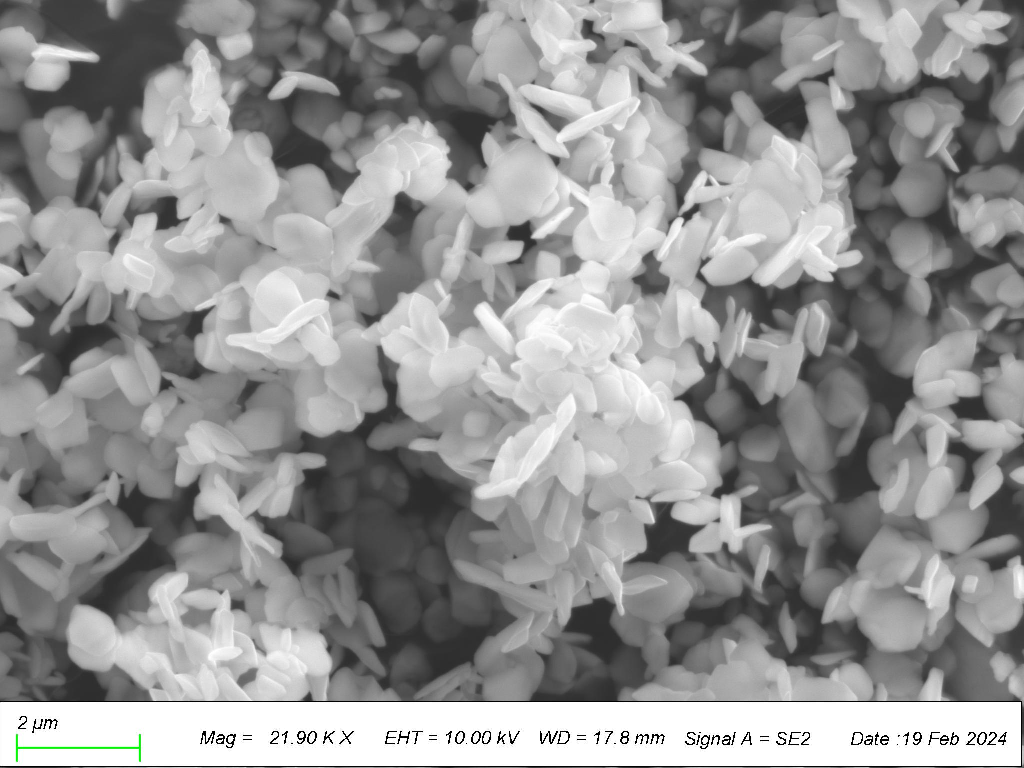
\includegraphics[width=\textwidth]{goe_pig_treatedRed19.pdf}
    \caption{Reacted (red) product}
    \label{fig:gt_pigment_red}
  \end{subfigure}\hfill
  \begin{subfigure}[t]{0.48\textwidth}
    \centering
    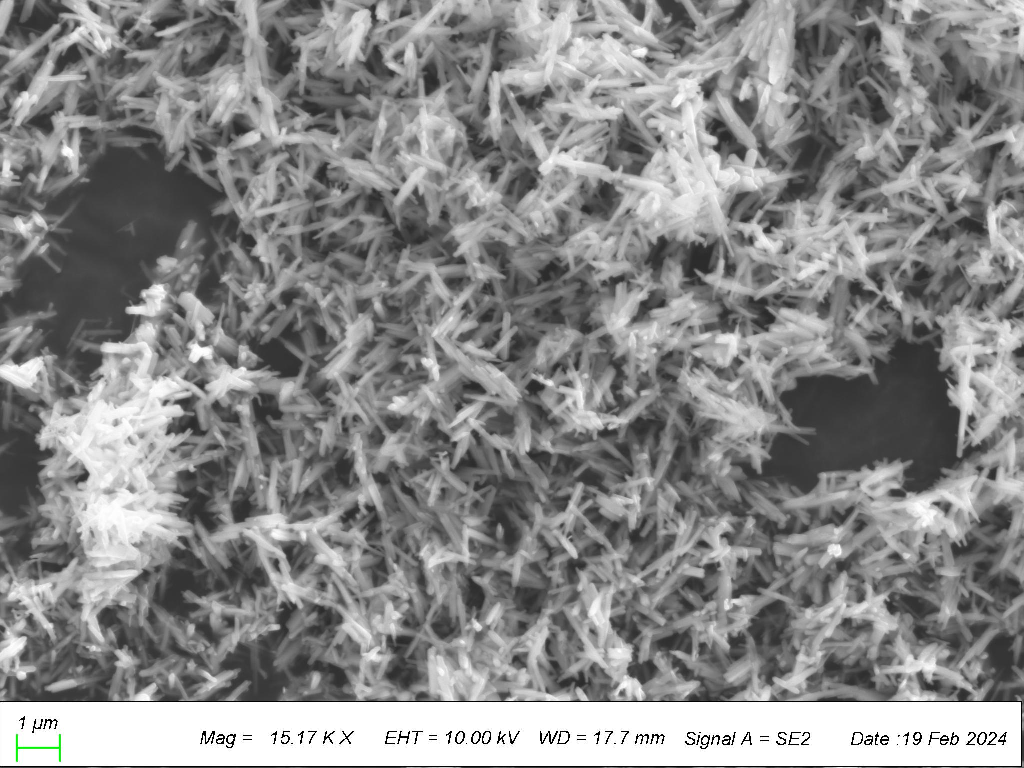
\includegraphics[width=\textwidth]{goe_pig_treatedYellow37.pdf}
    \caption{Unreacted (yellow) pigment}
    \label{fig:gt_pigment_yellow}
  \end{subfigure}
  \caption{Secondary electron images of synthetic goethite pigment after treatment at water vapor
  saturation and 200--250~$^\circ$C for about a day (\S\ref{sec:gt_pigment_methods}). (a) Material from a
  completely reacted (red) ampoule: the acicular goethite has been replaced by equant to platy hematite
  crystals $\sim$0.5--1~\textmu m across. (b) Material from an
  unreacted (yellow) ampoule, which retains the unchanged acicular habit of the starting pigment. The change
  in crystal habit requires dissolution of goethite and precipitation of hematite from the fluid,
  and the all-or-nothing outcome of the experiments indicates that the reaction is fast once it begins.}
  \label{fig:gt_pigment}
\end{figure}

Conversion either went to completion within a fluid-connected volume or did not occur at all, 
even where reacted and unreacted pigment shared the same ampoule and thermal history. We posit 
that the fluid-mediated reaction requires some threshold of dissolved Fe(III) in the fluid to 
nucleate hematite, but because the reaction consumes and produces dissolved Fe(III) in equal proportions, 
it is not self-limiting and proceeds quickly to completion once that threshold is reached. 

Grain size and bulk thermodynamics cannot explain why the pigment blades reacted when the natural 
polycrystalline goethite did not. At 1~\textmu m, the surface contribution to $\Delta G_r$ is only
$\sim$0.04~kJ, and the bulk driving force at saturation is the same 6--11~kJ for both materials
(Table~\ref{tab:gt_dmu}). The most likely difference is the fluid itself. Commercial iron-oxide
pigments are commonly produced by precipitation from iron-salt solutions. They can carry
residual soluble salts such as iron and alkali sulfates or nitrates, and they are often surface-treated with 
organometallic compounds \citep{legodi2007,almeidasilva2017,xu2021}. Such contaminants would
change the pH and ionic strength of the water they are heated in, and with them the solubility
of Fe(III). The dissolution--precipitation pathway is limited by how much iron the fluid
carries, so a modest increase in Fe(III) solubility could make a nucleation-limited reaction
viable. The natural Win-06-01b goethite, by contrast, was heated in
distilled water, where near-neutral Fe(III) solubility is very low, potentially offering an explanation for
the divergent outcomes.


\bibliographystyle{elsarticle-harv}
\bibliography{../../references,goethite_paper_extra}
\end{document}
